\documentclass[12pt,letterpaper]{article}
\usepackage[letterpaper,left=1.00in,right=1.00in,top=0.87in,bottom=0.85in]{geometry}
\usepackage{fontspec}
\usepackage{amsmath,unicode-math}
\usepackage{microtype}
\usepackage{xcolor,booktabs,array,tabularx,tikz}
\usepackage{hyperref}
\setmainfont{Latin Modern Roman}
\setsansfont{Latin Modern Sans}
\setmathfont{Latin Modern Math}
\definecolor{Ink}{HTML}{182633}
\definecolor{Muted}{HTML}{445562}
\definecolor{Accent}{HTML}{006C65}
\definecolor{Rule}{HTML}{B6C8CB}
\definecolor{Pale}{HTML}{EEF5F4}
\definecolor{PaperBlue}{HTML}{E5EFF6}
\hypersetup{colorlinks=true,linkcolor=Accent,pdftitle={Ten Problems That Teach Calculus},pdfsubject={Ten expanded worked solutions in single-variable calculus},pdfdisplaydoctitle=true,bookmarksopen=true}
\setlength{\parindent}{0pt}
\setlength{\parskip}{6pt plus 0.5pt}
\linespread{1.12}
\setlength{\emergencystretch}{1em}
\setlength{\abovedisplayskip}{8pt}
\setlength{\belowdisplayskip}{8pt}
\setlength{\abovedisplayshortskip}{6pt}
\setlength{\belowdisplayshortskip}{7pt}
\pagestyle{empty}
\raggedbottom
\newcommand{\folio}[1]{\par\vfill\noindent{\color{Rule}\rule{\linewidth}{0.55pt}}\par
  \vspace{1pt}\noindent{\sffamily\small\color{Muted}Ten Problems That Teach Calculus}\hfill
  {\sffamily\small\bfseries\color{Accent}#1}\par}
\newcommand{\eyebrow}[1]{{\sffamily\bfseries\footnotesize\color{Accent}\addfontfeatures{LetterSpace=9}#1}\par}
\newcommand{\problem}[4]{\clearpage\pdfbookmark[1]{#1. #3}{p#1}%
  \eyebrow{PROBLEM #1 \enspace / \enspace #2}
  \vspace{4pt}
  {\fontsize{28}{31}\selectfont\bfseries #3\par}
  \vspace{6pt}\noindent{\color{Rule}\rule{\linewidth}{0.55pt}}\par
  {\color{Muted}\itshape #4\par}\vspace{3pt}}
\newcommand{\answer}[1]{\par\noindent\colorbox{Pale}{%
  \begin{minipage}{\dimexpr\linewidth-2\fboxsep\relax}
  \vspace{4pt}\noindent\hspace{6pt}\begin{minipage}{\dimexpr\linewidth-12pt\relax}
  {\sffamily\bfseries\small\color{Accent}ANSWER}\enspace #1
  \end{minipage}\vspace{4pt}
  \end{minipage}}\par\vspace{4pt}}
\newcommand{\step}[1]{\par\vspace{3pt}{\sffamily\bfseries\color{Accent}#1}\par\nobreak}
\newcommand{\idea}[1]{\par\vspace{5pt}{\color{Muted}\textbf{Takeaway.} #1}\par}
\newcommand{\linkrow}[4]{\hyperlink{p#1.1}{\textsf{\textbf{#1}}} & \hyperlink{p#1.1}{#2} & \textcolor{Muted}{\small #3} & \textsf{#4}\\[4pt]}
\newcommand{\uom}[1]{\,\mathrm{#1}}
\begin{document}
\color{Ink}
\pdfbookmark[0]{Contents}{top}
\eyebrow{A SINGLE-VARIABLE CALCULUS READER}
\vspace{14pt}
{\fontsize{46}{48}\selectfont\bfseries Ten Problems\\That Teach Calculus\par}
\vspace{8pt}
{\fontsize{19}{22}\selectfont\itshape\color{Muted}Expanded worked solutions\par}
\vspace{12pt}
\noindent{\color{Accent}\rule{48pt}{2pt}}\par
\vspace{9pt}
If ten problems had to stand in for a course, each would need to teach a move worth using again. These solutions begin with the situation, identify the move that makes it tractable, and finish by interpreting the answer or checking its accuracy.
\vspace{8pt}

\eyebrow{CONTENTS}
\vspace{2pt}
{\setlength{\tabcolsep}{5pt}\renewcommand{\arraystretch}{1.10}
\begin{tabularx}{\linewidth}{@{}>{\centering\arraybackslash}p{0.32in} >{\raggedright\arraybackslash}X >{\raggedright\arraybackslash}p{2.20in} r@{}}
\toprule
\textsf{\small No.} & \textsf{\small Problem} & \textsf{\small Main idea} & \textsf{\small Page}\\
\midrule
\linkrow{01}{Oscillating near zero}{The squeeze theorem}{2}
\linkrow{02}{Speed at one instant}{The derivative from a limit}{3}
\linkrow{03}{The sliding ladder}{Related rates}{4}
\linkrow{04}{The largest open-top box}{Constrained optimization}{5}
\linkrow{05}{Estimating an exponential}{Taylor approximation}{6}
\linkrow{06}{How far did the cart travel?}{Signed accumulation}{7}
\linkrow{07}{The moving edge of an integral}{The Fundamental Theorem}{8}
\linkrow{08}{A finite total over infinite time}{Improper integrals}{9}
\linkrow{09}{Predicting how coffee cools}{Differential equations}{10}
\linkrow{10}{How many terms are enough?}{Series and error bounds}{11}
\bottomrule
\end{tabularx}}

\vspace{16pt}
{\color{Muted}\textbf{A way to read this.} Before following each solution, predict the direction, sign, or rough size of the answer. Then see which parts of your prediction the mathematics confirms.}
\folio{01}

\problem{01}{LIMITS}{Oscillating near zero}{Compare the behavior of \(\sin(1/x)\) and \(x\sin(1/x)\) as \(x\) approaches zero. Can either function be made continuous at zero by assigning it a value there?}
\answer{\(\sin(1/x)\) has no limit at zero. The limit of \(x\sin(1/x)\) is \(0\), so defining the second function to be \(0\) at zero makes it continuous there.}

\step{Find two ways to approach zero.}
For the first function, consider two sequences of positive \(x\)-values:
\[
  x_n=\frac{1}{\pi/2+2\pi n},
  \qquad
  y_n=\frac{1}{3\pi/2+2\pi n}.
\]
Both approach zero as \(n\to\infty\). But \(\sin(1/x_n)=1\) for every \(n\), whereas \(\sin(1/y_n)=-1\) for every \(n\). Even from the right, the function approaches different values along different sequences. No choice of value at \(x=0\) can fix that.

\step{Bound the height of the oscillations.}
Multiplication by \(x\) does not stop the oscillation. It does make the oscillations smaller, because \(|\sin(1/x)|\leq 1\). For \(x\ne 0\),
\[
  \bigl|x\sin(1/x)\bigr|\leq |x|,
  \qquad\text{so}\qquad
  -|x|\leq x\sin(1/x)\leq |x|.
\]
Both outer expressions tend to zero as \(x\to0\). By the squeeze theorem, the expression between them tends to zero too.

\idea{A limit concerns values nearby. An oscillation can continue indefinitely while its amplitude shrinks to zero.}
\folio{02}

\problem{02}{DERIVATIVES}{Speed at one instant}{A cart has position \(s(t)=t^2\) meters, with \(t\) in seconds. Find its instantaneous velocity at \(t=3\) by taking a limit of average velocities. Do not use the power rule.}
\answer{The instantaneous velocity at \(t=3\) is \(6\uom{m/s}\).}

\step{Start with an average velocity you could measure.}
Measure the position at \(t=3\) and again at \(t=3+h\). Divide the change in position by the change in time. For \(h\ne0\),
\begin{align*}
\frac{s(3+h)-s(3)}{h}
 &=\frac{(3+h)^2-9}{h}\\
 &=\frac{6h+h^2}{h}\\
 &=6+h.
\end{align*}
If \(h\) is positive, the second reading comes after \(3\) seconds. If \(h\) is negative, it comes before. In either case the quotient gives the average velocity over the interval between the readings.

\step{Shrink the interval from both sides.}
For example, \(h=0.1\) gives \(6.1\uom{m/s}\), while \(h=-0.1\) gives \(5.9\uom{m/s}\). As either interval shrinks,
\[
   s'(3)=\lim_{h\to0}\frac{s(3+h)-s(3)}{h}
         =\lim_{h\to0}(6+h)=6\uom{m/s}.
\]
We never divide by zero. We simplify for nonzero \(h\), then ask what those average velocities approach.

\idea{An instantaneous rate is a limit of rates measured over intervals. For a position graph, the slopes of the secant lines approach the slope of the tangent.}
\folio{03}

\problem{03}{RELATED RATES}{The sliding ladder}{A 10-foot ladder leans against a wall. Its foot slides outward at \(1\uom{ft/s}\). Predict whether the top is moving faster or slower than the foot when the foot is 6 feet out, then calculate its velocity.}
\answer{The top is moving downward at \(0.75\uom{ft/s}\), slower than the foot is moving outward.}

\step{Use the fixed length to connect the two positions.}
Let \(x\) be the foot's distance from the wall and \(y\) the top's height. The right triangle gives \(x^2+y^2=100\). When \(x=6\), \(y=8\). A small change in \(y\) has a larger effect on \(y^2\) at \(8\) than the same change in \(x\) has on \(x^2\) at \(6\). So the top needs less motion to offset the foot's motion at that moment.

\begin{center}
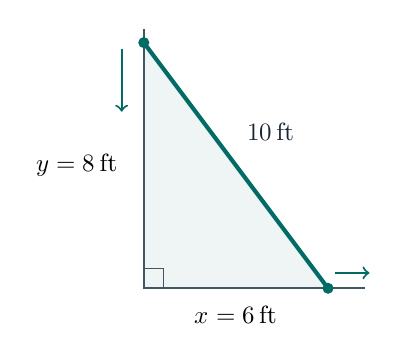
\begin{tikzpicture}[x=.39cm,y=.39cm,font=\small]
\draw[fill=Pale,draw=none] (0,0)--(6,0)--(0,8)--cycle;
\draw[draw=Muted,line width=.8pt] (0,8.45)--(0,0)--(7.2,0);
\draw[draw=Muted] (0,.64)--(.64,.64)--(.64,0);
\draw[draw=Accent,line width=1.5pt] (0,8)--(6,0) node[pos=.47,above right=2pt,text=Ink] {\(10\uom{ft}\)};
\fill[Accent] (0,8) circle (2pt) (6,0) circle (2pt);
\node[below=3pt] at (3,0) {\(x=6\uom{ft}\)};
\node[left=6pt] at (0,4) {\(y=8\uom{ft}\)};
\draw[->,draw=Accent,line width=.75pt] (-.72,7.8)--(-.72,5.75);
\draw[->,draw=Accent,line width=.75pt] (6.22,.5)--(7.35,.5);
\end{tikzpicture}
\end{center}

\step{Differentiate the constraint with respect to time.}
Both \(x\) and \(y\) change with time, so the chain rule gives
\[
  2x\frac{dx}{dt}+2y\frac{dy}{dt}=0,
  \qquad
  \frac{dy}{dt}=-\frac{x}{y}\frac{dx}{dt}
              =-\frac68(1)=-0.75\uom{ft/s}.
\]
The minus sign means the height is decreasing. The rate ratio depends on the ladder's position. As the ladder gets flatter, \(x/y\) grows.

\idea{When a constraint links changing quantities, differentiate the constraint before plugging in the numbers for one instant.}
\folio{04}

\problem{04}{OPTIMIZATION}{The largest open-top box}{Cut equal squares from the four corners of a \(12\)-by-\(20\)-inch sheet. Fold up the sides. What cut size gives the largest volume, and how do you know it is the largest?}
\answer{Cut squares of side \(\dfrac{16-2\sqrt{19}}{3}\) inches, approximately \(2.43\) inches.}

\step{Turn the construction into a function.}
If the corner squares have side length \(x\), the box has height \(x\). Two cuts shorten each sheet dimension, leaving a base \(12-2x\) inches wide and \(20-2x\) inches long. Thus
\[
  V(x)=x(12-2x)(20-2x)
      =240x-64x^2+4x^3.
\]
A usable box requires \(0<x<6\). For comparison, include the collapsed cases \(x=0\) and \(x=6\), both of which give volume zero.

\step{Find the interior candidates.}
Since \(V\) is differentiable, an interior maximum must satisfy
\[
  V'(x)=240-128x+12x^2=0.
\]
The quadratic formula gives
\[
  x=\frac{16-2\sqrt{19}}{3}\approx2.43
  \qquad\text{or}\qquad
  x=\frac{16+2\sqrt{19}}{3}\approx8.24.
\]
The second root is outside the allowable interval. A cut that large would exceed half the sheet's width.

\step{Check that the remaining candidate is the global maximum.}
The volume function is continuous on \([0,6]\), so it attains a maximum there. The endpoints give zero, and every cut between them yields a positive volume. Thus the maximum must be interior, and the only admissible critical point is the answer.

\idea{A zero derivative supplies a candidate. The physical domain and the endpoint check establish that it is the best one.}
\folio{05}

\problem{05}{TAYLOR APPROXIMATION}{Estimating an exponential}{Without a calculator, estimate \(e^{-0.1}\) using the value, slope, and second derivative of \(e^x\) at zero. Give a bound on the error.}
\answer{\(e^{-0.1}\approx 0.905\), with absolute error less than \(0.000167\). The estimate is slightly high.}

\step{Match the value, slope, and second derivative.}
For \(f(x)=e^x\), we have \(f(0)=f'(0)=f''(0)=1\). The quadratic Taylor polynomial therefore is
\[
  P_2(x)=f(0)+f'(0)x+\frac{f''(0)}{2!}x^2
        =1+x+\frac{x^2}{2}.
\]
At \(x=-0.1\), this gives
\[
  P_2(-0.1)=1-0.1+\frac{0.01}{2}=0.905.
\]

\step{Bound what the polynomial left out.}
Taylor's theorem says that, for some \(\xi\) between \(-0.1\) and \(0\),
\[
  e^{-0.1}-P_2(-0.1)
      =\frac{f'''(\xi)}{3!}(-0.1)^3
      =\frac{e^\xi}{6}(-0.1)^3.
\]
Here \(0<e^\xi\leq1\). The remainder is negative and its magnitude is bounded by
\[
  \bigl|e^{-0.1}-0.905\bigr|
  \leq \frac{0.001}{6}<0.000167.
\]
The negative remainder explains why the quadratic approximation is an overestimate.

\idea{Local information makes a prediction. A bound on the next derivative tells you how much to trust it.}
\folio{06}

\problem{06}{DEFINITE INTEGRALS}{How far did the cart travel?}{A cart's velocity is \(v(t)=t^2-1\) meters per second for \(0\leq t\leq2\). Sketch the velocity, build the displacement as a limit of sums, and find the total distance.}
\answer{The cart covers \(2\uom{m}\) and ends up \(\tfrac23\uom{m}\) forward of its starting point.}

\step{Read the direction from the sign of velocity.}
The cart moves backward until \(t=1\), when the velocity changes sign. It then moves forward. The signed areas in the velocity graph represent the two legs of the trip.

\begin{center}
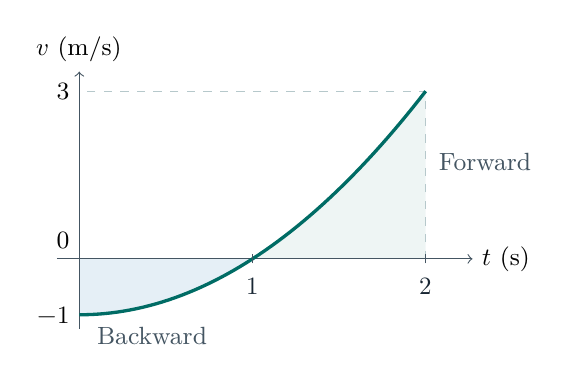
\begin{tikzpicture}[x=2.2cm,y=.71cm,font=\small]
\fill[PaperBlue] (0,0) -- plot[domain=0:1,samples=25] (\x,{\x*\x-1}) -- cycle;
\fill[Pale] (1,0) -- plot[domain=1:2,samples=30] (\x,{\x*\x-1}) -- (2,0) -- cycle;
\draw[->,draw=Muted] (-.13,0)--(2.27,0) node[right] {\(t\) (s)};
\draw[->,draw=Muted] (0,-1.25)--(0,3.35) node[above] {\(v\) (m/s)};
\draw[draw=Rule,dashed] (2,0)--(2,3)--(0,3);
\draw[draw=Accent,line width=1.2pt] plot[domain=0:2,samples=55] (\x,{\x*\x-1});
\foreach \x in {1,2}{\draw[draw=Muted] (\x,-.08)--(\x,.08) node[below=5pt,text=Ink] {\(\x\)};}
\node[above left] at (0,0) {0};
\node[left] at (0,-1) {\(-1\)};
\node[left] at (0,3) {3};
\node[below,text=Muted] at (.42,-1.04) {Backward};
\node[right,text=Muted] at (2.02,1.73) {Forward};
\end{tikzpicture}
\end{center}

\step{Add the small signed changes in position.}
Split the time into \(n\) pieces of width \(\Delta t=2/n\). With a sample time \(t_i^*\) in each piece, \(v(t_i^*)\Delta t\) approximates the change in position on that piece. Taking the limit gives
\[
  \lim_{n\to\infty}\sum_{i=1}^{n}v(t_i^*)\Delta t
      =\int_0^2 (t^2-1)\,dt.
\]
With antiderivative \(t^3/3-t\), evaluation from \(0\) to \(1\) gives \(-\tfrac23\uom{m}\), and from \(1\) to \(2\) gives \(+\tfrac43\uom{m}\). Add with signs for displacement, \(\tfrac23\uom{m}\). Add the magnitudes for distance, \(2\uom{m}\).

\idea{Integrate velocity for net change in position. Integrate speed, \(|v|\), for total ground covered.}
\folio{07}

\problem{07}{FUNDAMENTAL THEOREM}{The moving edge of an integral}{Let \(A(x)=\int_0^{x^2}\cos(t^2)\,dt\). Find \(A'(x)\) without evaluating the integral, and explain what happens when \(x\) increases a little.}
\answer{\(A'(x)=2x\cos(x^4)\).}

\step{Ask how the total changes when the edge moves.}
First let the upper limit be a separate variable \(u\) and define
\[
   G(u)=\int_0^u\cos(t^2)\,dt.
\]
The integrand is continuous. The Fundamental Theorem of Calculus gives \(G'(u)=\cos(u^2)\), its value right at the upper edge.

\step{Account for how fast the edge moves.}
Our original function is \(A(x)=G(x^2)\). The edge is at \(u=x^2\), so it moves at rate \(du/dx=2x\). By the chain rule,
\[
  A'(x)=G'(x^2)\,\frac{d}{dx}(x^2)
       =\cos\bigl((x^2)^2\bigr)\cdot 2x
       =2x\cos(x^4).
\]

\step{Picture the extra piece as a thin signed strip.}
A small increase \(\Delta x\) moves the edge by
\[
  (x+\Delta x)^2-x^2=2x\,\Delta x+(\Delta x)^2.
\]
To first order, the strip has signed width \(2x\,\Delta x\) and height \(\cos(x^4)\). For negative \(x\), a small increase in \(x\) actually moves the upper edge to the left. The sign of \(2x\) accounts for that.

\idea{You do not need the total already accumulated to find its current rate of change. For a moving upper limit, multiply the integrand's value at the edge by the edge's velocity.}
\folio{08}

\problem{08}{IMPROPER INTEGRALS}{A finite total over infinite time}{Water enters a tank at rate \(t e^{-t}\) liters per minute, with \(t\) measured in minutes. How much water enters over all time? Why is it not enough to know the rate tends to zero?}
\answer{Exactly \(1\) liter enters the tank over all time.}

\step{Accumulate the water up to a finite time.}
Use integration by parts with \(u=t\) and \(dv=e^{-t}\,dt\), so \(du=dt\) and \(v=-e^{-t}\). The volume added by time \(T\) is
\begin{align*}
  \int_0^T t e^{-t}\,dt
    &=\bigl[-t e^{-t}\bigr]_0^T+\int_0^T e^{-t}\,dt\\
    &=\bigl[-(t+1)e^{-t}\bigr]_0^T\\
    &=1-(T+1)e^{-T}.
\end{align*}

\step{Take the limit of those finite totals.}
The exponential in the denominator grows faster than the linear numerator, so \((T+1)e^{-T}=(T+1)/e^T\to0\). For example, applying L'Hôpital's rule to that quotient gives the same limit as \(1/e^T\). Hence
\[
  \int_0^\infty t e^{-t}\,dt
    :=\lim_{T\to\infty}\int_0^T t e^{-t}\,dt
    =1.
\]

\step{Compare with a rate that shrinks too slowly.}
The rate \(1/(1+t)\) also tends to zero, but its accumulated total is
\[
   \int_0^T \frac{dt}{1+t}=\ln(1+T)\longrightarrow\infty.
\]
Both rates get small. Only the first one gets small fast enough to give a finite total.

\idea{An improper integral is a limit of ordinary integrals. Check the limiting total, not just the limiting rate.}
\folio{09}

\problem{09}{DIFFERENTIAL EQUATIONS}{Predicting how coffee cools}{Coffee starts at \(90^\circ\mathrm{C}\) in a \(20^\circ\mathrm{C}\) room. It is \(60^\circ\mathrm{C}\) after ten minutes. Assume its cooling rate is proportional to how much hotter it is than the room. When will it reach \(40^\circ\mathrm{C}\)?}
\answer{The model predicts \(40^\circ\mathrm{C}\) about \(22.4\) minutes after the start.}

\step{Write a rule for the excess temperature.}
Let \(T(t)\) be the coffee temperature and \(E(t)=T(t)-20\) its excess above room temperature. With \(t\) in minutes, the model is
\[
   \frac{dE}{dt}=-kE,\qquad k>0,\qquad E(0)=70.
\]
The negative sign expresses cooling. While \(E>0\), dividing by \(E\) gives \(d(\ln E)/dt=-k\). Integrating from time zero gives \(\ln(E/70)=-kt\), or
\[
  E(t)=70e^{-kt}.
\]

\step{Use the ten-minute reading to fit the model.}
At \(t=10\), the coffee is \(40^\circ\) above the room temperature. Therefore
\[
  40=70e^{-10k}
  \qquad\Longrightarrow\qquad
  k=\frac{\ln(7/4)}{10}\uom{min^{-1}}.
\]

\step{Solve for when the excess reaches \(20^\circ\).}
The target is \(40^\circ\mathrm C\), or \(20^\circ\) above the room. In the fitted model,
\[
   20=70e^{-kt}
   \qquad\Longrightarrow\qquad
   t=\frac{10\ln(7/2)}{\ln(7/4)}\uom{min}
     \approx22.4\uom{min}.
\]

\idea{The ten-minute measurement fits the model. An additional measurement would test its prediction. These are different jobs.}
\folio{10}

\problem{10}{SERIES AND ERROR BOUNDS}{How many terms are enough?}{Integrate the finite geometric sum \(1-x+x^2-\cdots\) from 0 to 1 to build the alternating series for \(\ln 2\). How many terms guarantee error less than \(0.001\)?}
\answer{The usual alternating-series bound guarantees the accuracy with \(999\) terms. The actual minimum is \(500\) terms.}

\step{Keep the remainder of the finite sum.}
The finite geometric identity, with its remainder included, is
\[
  \frac{1}{1+x}=\sum_{k=0}^{N-1}(-x)^k+\frac{(-x)^N}{1+x}.
\]
Integrate each side over \([0,1]\). If \(S_N=1-\tfrac12+\tfrac13-\cdots+\tfrac{(-1)^{N-1}}{N}\), then
\[
  \ln 2-S_N=(-1)^N\int_0^1\frac{x^N}{1+x}\,dx.
\]
The integral is the absolute error. Because \(1/(1+x)<1\) for \(x>0\), the error is strictly less than \(1/(N+1)\), the magnitude of the first omitted term. This bound tends to zero, establishing that the series sums to \(\ln 2\). It also guarantees the requested accuracy at \(N=999\).

\step{Tighten the bound to find the first term count that works.}
For \(0<x<1\), we have \(\tfrac12<1/(1+x)<1-x/2\). The upper inequality follows from \((1-x/2)(1+x)=1+x(1-x)/2>1\). Multiply by \(x^N\) and integrate:
\[
  \frac{1}{2(N+1)}
    <\bigl|\ln 2-S_N\bigr|
    <\frac{1}{N+1}-\frac{1}{2(N+2)}.
\]
At \(N=499\), the lower bound is exactly \(0.001\), so \(499\) terms do not suffice. At \(N=500\), the upper bound is
\[
  \frac{1}{501}-\frac{1}{1004}
    =\frac{503}{503004}<\frac{1}{1000}.
\]
The error decreases with \(N\), since \(x^N\) decreases with \(N\) for \(0<x<1\). Therefore \(500\) is the first term count that works.

\idea{Convergence says the approximation will eventually be good enough. An error bound tells you when you can stop.}
\folio{11}
\end{document}
